%% question-2.tex
%%

%% ==============================
\subsection{Version enrichie du diagramme de classe du jeu}
\label{sec:question-2}
%% ==============================

Dans cette version du diagramme de classe \ref{fig:Jeu}, la classe Jeu est est maintenant associée a deux nouvelles classes.

La classe \emph{ProfilUtilisateur}, qui sauvegarde le profil de chaque utilisateur et qui est elle même associée a \emph{HistoriqueDeNiveau} d'une part
et d'autre part à \emph{Lesson}, par la classe d'association \emph{Reussite}, qui donne le nombre de lessons réussies.
Et la classe \emph{Editeur} qui permet d'éditer un \emph{Niveau} à la fois. 

Cette classe \emph{Editeur} est en assiciation avec \emph{ElementNiveau}
car il est possible d'éditer un niveau (et donc d'avoir besoins des éléments pour construire un niveau) sans avoir de lessons et de niveau existants.

\emph{ProfilUtilisateur} est aussi associé à niveau car il faut pouvoir conserver les niveaux édités par l'utilisateur et à \emph{NiveauEnCours} car il
faut pouvoir conserver les données de performances de chaque niveau. 

La composition se trouvant entre \emph{Niveau} et \emph{NiveauEnCours} est présente
car il faut un \emph{Niveau} pour avoir un \emph{NiveauEnCours}. La classe \emph{NiveauEnCours} est associée via la classe d'association \emph{PositionJoueur}
à \emph{Joueur} car étant donné que Cody peut se déplacer sur le niveau, il faut pourvoir connaître sa position via \emph{getElementAtPosition}.

La classe \emph{Niveau} est quand à elle associée par une assiciation 1-1 à \emph{Joueur} et \emph{Coffre} car il ne peut y avoir qu'un seul joueur et un
seul coffre par \emph{Niveau}. 

Elle est aussi associée à \emph{ElementNiveau} qui possède 4 enfants directs (\emph{Surface},
\emph{Personnage},\emph{Obstacle} et \emph{Teleporteur}).

\emph{Surface} a comme enfants (\emph{Sol},\emph{Pont} et \emph{Coffre}), \emph{Personnage} a (\emph{Joueur} et \emph{Ennemi}) et \emph{Teleporteur} a
(\emph{Tunnel} et \emph{Levier}). 

Pour la classe \emph{Sol}, le changement de \emph{décors} se fait via une énumération \emph{Theme}. 

Dans la classe \emph{Ennemi}, le boolean \emph{reaction} permet d'avoir des ennemis agressifs ou non. La classe \emph{Tunnel} est en double association sur elle même car il y a une entrée et une
sortie. 

Dans le cas contraire , la variable\emph{isOpen} est a false et il n'y a qu'un tunnel fermé. Un \emph{Tunnel} lorsqu'il est double ( une entrée et une sortie)
est en assiciation 1-1 avec un \emph{Levier} qui permet de l'ouvrir.


\begin{sidewaysfigure}
    \centering
	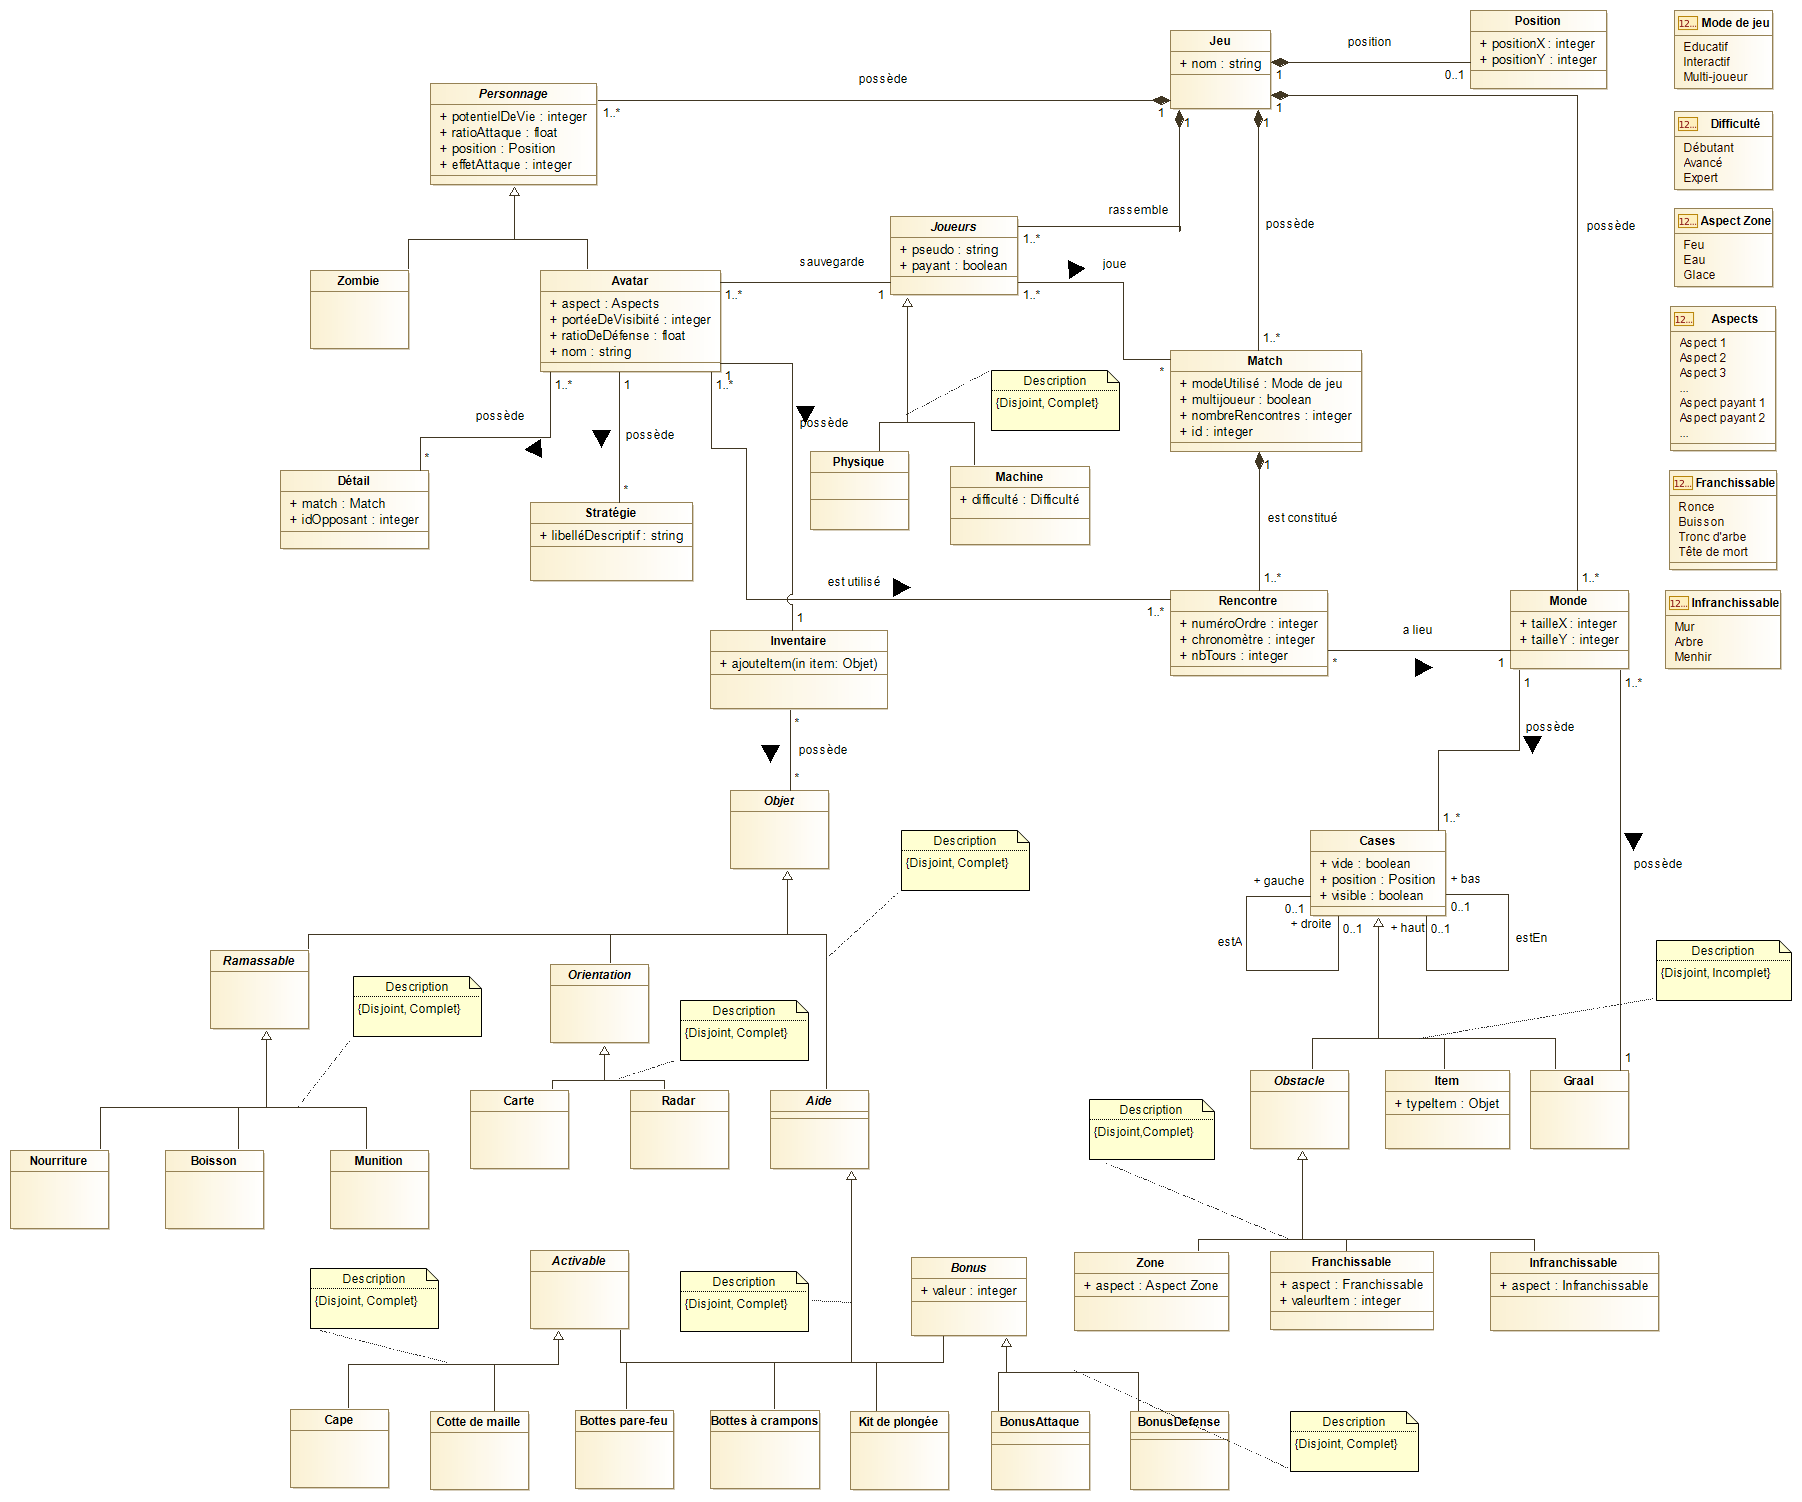
\includegraphics[width=\textwidth]{assets/Jeu}
	\caption{Diagramme enrichit}
	\label{fig:Jeu}
\end{sidewaysfigure}

\newpage